%----------------------------------------------------------------------------------------
%	HASIL DAN PEMBAHASAN
%----------------------------------------------------------------------------------------
\section*{HASIL DAN PEMBAHASAN}
\subsection*{Fase Analisis}
\begin{flushleft}
Model Ontologi
\end{flushleft}
Pada penelitian ini ontologi yang digunakan adalah Gene Ontology (GO).  Struktur ontologi dari GO berupa struktur \textit{graph}. Pada struktur ontologi ini terms merupakan \textit{node}-nya dan relasi antar \textit{terms} tersebut merupakan \textit{edge}-nya. Setiap \textit{terms} atau \textit{node} yang terdapat pada GO memiliki definisi masing-masing, begitu juga dengan relasi atau \textit{edge}. Pada GO terdapat beberapa jenis relasi yaitu \textit{is a}, \textit{part of}, \textit{has part} dan \textit{regulates}.
\begin{flushleft}
\textbf{Ruang Lingkup}
\end{flushleft}
GO memiliki tiga domain yaitu \textit{cellular component}, \textit{molecular function} dan \textit{biological process}. Pada penelitian ini akan dibuat sistem yang dapat mencari dan merepresentasikan \textit{gene product}.
\begin{flushleft}
Relasi\par
1. \textit{is\_a}
\end{flushleft}\par
Relasi \textit{is a} adalah relasi paling sederhana yang terdapat pada GO. Relasi \textit{is a} dapat dikatakan seperti A \textit{is a} B, artinya adalah setiap kelas yang ada pada A merupakan bagian / \textit{sub class} dari B. Relasi ini digunakan untuk menunjukkan keterkaitan antara kelas yang lebih spesifik ke kelas yang lebih umum. Relasi \textit{is a} juga dapat menunjukkan inferensi antar kelas, sebagai contoh pada Gambar \ref{fig:is_a}  apabila A \textit{is a} B dan B \textit{is a} C maka dapat dikatakan bahwa A \textit{is a} C.

\begin{figure}[h!] % Gunakan \begin{figure*} untuk memasukkan Gambar
	\centering
	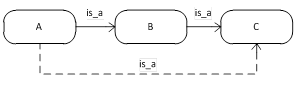
\includegraphics[width=200pt]{isa.png}
	\caption{Relasi \textit{is\_a}}
	\label{fig:is_a}
\end{figure}

Pada GO contoh dari relasi ini di tunjukkan seperti pada Gambar \ref{fig:contoh_is_a}. Terlihat bahwa \textit{single organism cellular process is a single organism process} dan \textit{single organism process is a biological process}, maka dari itu \textit{single organism cellular process is a biological process}.

\begin{figure}[h!] % Gunakan \begin{figure*} untuk memasukkan Gambar
	\centering
	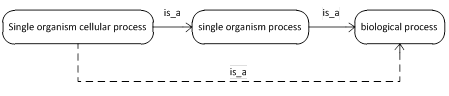
\includegraphics[width=200pt]{contoh_is_a.png}
	\caption{Contoh relasi \textit{is\_a}}
	\label{fig:contoh_is_a}
\end{figure}
\begin{flushleft}
	2. \textit{part\_of}
\end{flushleft}\par
Relasi \textit{part of}  ini menjelaskan bahwa apabila A \textit{part of} B, maka A merupakan salah satu kelas yang ada di dalam B. Relasi ini biasanya dipakai untuk menjelaskan suatu proses yang memiliki beberapa proses di dalamnya. Pada Gambar \ref{fig:part_of} menunjukkan hubungan \textit{part of} antara A dan B, sehingga apabila proses B tidak ada maka proses A pun tidak ada, tetapi apabila A tidak ada belum tentu B tidak ada.
\begin{figure}[h!] % Gunakan \begin{figure*} untuk memasukkan Gambar
	\centering
	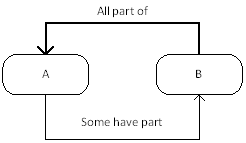
\includegraphics[width=200pt]{part_of.png}
	\caption{Relasi \textit{part\_of}}
	\label{fig:part_of}
\end{figure}
\par
Pada GO contoh relasi ini ditunjukkan seperti pada Gambar \ref{fig:contoh_part_of} yang menunjukkan bahwa \textit{mitochondrial membrane merupakan part of mitochondrion}.
\begin{figure}[h!] % Gunakan \begin{figure*} untuk memasukkan Gambar
	\centering
	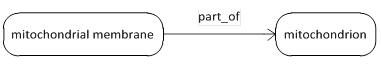
\includegraphics[width=200pt]{contoh_part_of.png}
	\caption{Contoh relasi \textit{part\_of}}
	\label{fig:contoh_part_of}
\end{figure}

\begin{flushleft}
3. \textit{has\_part}
\end{flushleft}\par
Relasi \textit{has part} merupakan kebalikan dari \textit{part of}. Apabila part of menunjukkan dari bagian kecil ke bagian yang lebih besar, maka \textit{has part} menunjukkan bagian besar memiliki bagian-bagian yang lebih kecil. Pada Gambar \ref{fig:has_part} menunjukkan skema relasi \textit{has part}, B memiliki bagian berupa A.
\begin{figure}[h!] % Gunakan \begin{figure*} untuk memasukkan Gambar
	\centering
	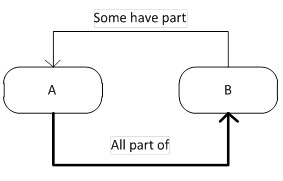
\includegraphics[width=200pt]{has_part.png}
	\caption{Relasi \textit{has\_of}}
	\label{fig:has_part}
\end{figure}
\par
Di dalam GO relasi ini ditunjukkan dengan hubungan antara \textit{nucleus} dengan \textit{chromosome} seperti terlihat pada Gambar \ref{fig:contoh_has_part}.
\begin{figure}[h!] % Gunakan \begin{figure*} untuk memasukkan Gambar
	\centering
	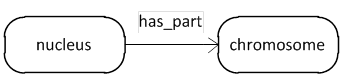
\includegraphics[width=200pt]{contoh_has_part.png}
	\caption{Contoh relasi \textit{has\_of}}
	\label{fig:contoh_has_part}
\end{figure}
\begin{flushleft}
4. \textit{regulates}
\end{flushleft}\par
Relasi \textit{regulates} merupakan relasi yang umum terdapat pada GO. Relasi ini menunjukkan bahwa node yang satu mempengaruhi node yang lain. Pada Gambar \ref{fig:regulates} menunjukkan bahwa B \textit{regulates} A, yang artinya apabila B merupakan suatu proses maka proses yang terjadi pada B akan mempengaruhi proses pada A, tetapi proses B tidak selalu terpengaruh dengan proses A.
\begin{figure}[h!] % Gunakan \begin{figure*} untuk memasukkan Gambar
	\centering
	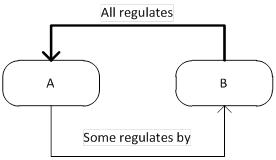
\includegraphics[width=200pt]{regulates.png}
	\caption{Relasi \textit{regulates}}
	\label{fig:regulates}
\end{figure}
\par
Relasi ini pada GO dicontohkan hubungan antara \textit{activation of reciprocal meiotic recombination} mempengaruhi proses dari \textit{meiotic cell cycle} yang ditunjukkan pada Gambar \ref{fig:contoh_regulates}.
\begin{figure}[h!] % Gunakan \begin{figure*} untuk memasukkan Gambar
	\centering
	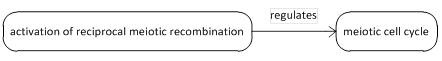
\includegraphics[width=200pt]{contoh_regulates.png}
	\caption{Contoh relasi \textit{regulates}}
	\label{fig:contoh_regulates}
\end{figure}
\begin{flushleft}
\textbf{Model Informasi}
\end{flushleft}
Setelah mendapatkan model ontologi dari GO maka tahap selanjutnya adalah merancang model informasi. Informasi yang akan ditampilkan kepada pengguna sistem adalah informasi yang terdapat pada GO akan ditampilkan dengan cara pengguna memasukkan kata kunci yang akan di cari. Kemudian setelah ditemukan untuk mengetahui lebih lanjut mengenai informasi dari hasil yang ditemukan maka pengguna dapat masuk ke halaman detail dengan menggunakan link yang ada pada hasil tersebut. Tabel \ref{tab:kelas} menunjukkan kelas yang ada di dalam sistem ini.

\begin{table}[h!]
	\footnotesize
	\caption{Kelas pada sistem GO}
	\centering
	\begin{tabulary}{0.47\textwidth}{LLL}
		\toprule
		\parbox{8em}{Kelas}&\parbox{8em}{Atribut} & Proses \\
		\midrule
		SearchForm & Keyword, Ontology & ViewForm()\par submitKeyword(string)\\
		Result & QueryResult &  viewQResult()\par viewOntology()\par viewDetail(string)
		\\
		\bottomrule
	\end{tabulary}
	\label{tab:kelas}
\end{table}

\begin{flushleft}
\textbf{Model User}
\end{flushleft}
Use Case sistem yang akan dibuat dapat dilihat pada Gambar \ref{fig:use_case}.
\begin{figure}[h!] % Gunakan \begin{figure*} untuk memasukkan Gambar
	\centering
	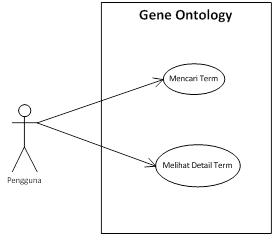
\includegraphics[width=200pt]{use_case.png}
	\caption{\textit{Use case diagram} sistem GO}
	\label{fig:use_case}
\end{figure}
\par
Pada use case ini menunjukkan bahwa pengguna dapat melakukan pencarian \textit{term} berdasarkan kata kunci yang ingin dicari. Kemudian setelah menemukan kata kunci yang dicari pengguna dapat melihat detail dari kata kunci tersebut.

Berdasarkan \textit{use case} pada Gambar \ref{fig:act1} maka dibuat \textit{activity diagram} untuk \textit{use case} mencari \textit{term} dan Gambar \ref{fig:act2} untuk \textit{use case} melihat \textit{detail term}. 

\begin{figure}[h!] % Gunakan \begin{figure*} untuk memasukkan Gambar
	\centering
	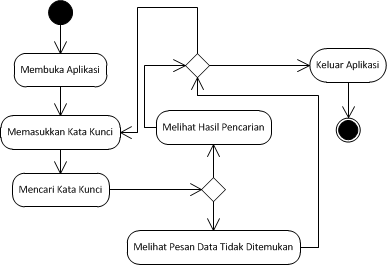
\includegraphics[width=100pt]{act1.png}
	\caption{\textit{Activity diagram} mencari term}
	\label{fig:act1}
\end{figure}

\begin{figure}[h!] % Gunakan \begin{figure*} untuk memasukkan Gambar
	\centering
	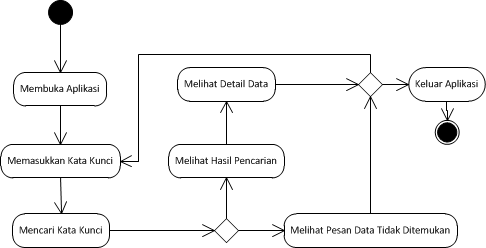
\includegraphics[width=100pt]{act2.png}
	\caption{\textit{Activity diagram} melihat detail term}
	\label{fig:act2}
\end{figure}

Dari \textit{activity diagram} yang dibuat maka dapat dibuat \textit{sequence diagram}. \textit{Sequence diagram} ini menunjukkan langkah detail yang akan dilakukan pengguna pada saat menggunakan sistem ini. Pada Gambar \ref{fig:sequence_1} menunjukkan \textit{sequence diagram} untuk \textit{use case} mencari \textit{term} dan Gambar \ref{fig:sequence_2} \textit{sequence diagram} untuk \textit{use case} melihat detail \textit{term}.
\begin{figure}[h!] % Gunakan \begin{figure*} untuk memasukkan Gambar
	\centering
	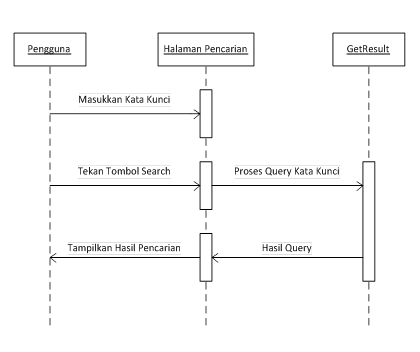
\includegraphics[width=200pt]{sequence_1.png}
	\caption{\textit{Sequence diagram} mencari \textit{term}}
	\label{fig:sequence_1}
\end{figure}
\begin{figure}[h!] % Gunakan \begin{figure*} untuk memasukkan Gambar
	\centering
	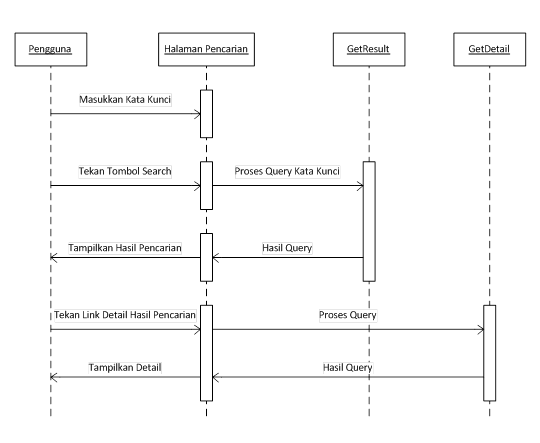
\includegraphics[width=200pt]{sequence_2.png}
	\caption{\textit{Sequence diagram} melihat detail \textit{term}}
	\label{fig:sequence_2}
\end{figure}
\subsection*{Fase Implementasi dan Desain}
\begin{flushleft}
\textbf{Parsing Ontologi}
\end{flushleft}
Ontologi merupakan salah satu cara yang digunakan untuk merepresentasikan pengetahuan. Ontologi menggunakan Uniform Resource Identifier (URI) untuk membentuk struktur dokumennya. URI ini digunakan untuk memberikan keterangan pada suatu objek. Objek dari ontologi terdiri dari tiga bagian yang disebut \textit{triples}. \textit{Triples} ini terdiri dari\textit{ subject}, \textit{predicate} dan \textit{object}. Tujuan dari dilakukan \textit{parsing} ontologi adalah untuk membuat ontologi dapat dibaca dan dipahami oleh pembuat sistem.

Model  data ontologi yang digunakan pada penelitian ini menggunakan RDF. RDF berisi kumpulan kumpulan \textit{triples} yang disimpan dalam format XML. Model data ini dipilih karena merupaka model data yang menjadi standar pada ontolgi, sehingga terdapat banyak \textit{parser} yang dapat melakukan parsing terhadap data RDF.

Parser yang digunakan pada penelitian ini adalah RDFLib. RDFLib merupakan package dari bahasa pemrograman python yang dapat melakukan \textit{parsing} terhadap data ontologi.  RDFLib dipilih karena memiliki beberapa kelebihan, seperti dapat mem-parsing berbagai jenis model data, dapat menyimpan graph dari suatu ontologi, dapat menyimpan data pada \textit{memory} maupun secara presistent, dan dapat menggunakan SPARQL untuk melakukan operasi pada data ontologi.

Untuk penggunaan RDFLib pada python maka sistem harus memanggil package RDFLib tersebut dengan syntax seperti pada Gambar \ref{fig:import}.

\begin{figure}[h!] % Gunakan \begin{figure*} untuk memasukkan Gambar
	\centering
	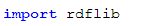
\includegraphics[width=100pt]{import.png}
	\caption{Pemanggilan \textit{package} RDFLib}
	\label{fig:import}
\end{figure}

Untuk melakukan parsing terhadap data ontologi maka syntax yang diperlukan seperti pada Gambar \ref{fig:parsing}. Pada Gambar \ref{fig:parsing} terlihat bahwa RDFLib melakukan parsing terhadap data ontology GO.

\begin{figure}[h!] % Gunakan \begin{figure*} untuk memasukkan Gambar
	\centering
	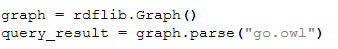
\includegraphics[width=200pt]{parsing.png}
	\caption{Proses \textit{parsing} ontologi}
	\label{fig:parsing}
\end{figure}

\begin{flushleft}
	\textbf{Implementasi Model Informasi}
\end{flushleft}

Pada proses implementasi model informasi maka dibuat \textit{user interface} yang akan digunakan oleh pengguna. Penelitian ini akan menghasilkan sistem yang berbasis web dengan menggunakan \textit{web framework} Flask yang merupakan \textit{web framework} python yang ringan. Pembuatan halaman web menggunakan HTML. Dengan dibuat sistem yang berbasis web maka sistem ini dapat dibuka di komputer manapun tanpa melakukan proses instalasi. Halaman yang dibuat pada sistem ini ditunjukkan pada Tabel \ref{tab:info}.

\begin{table}[h!]
	\footnotesize
	\caption{Halaman yang dibuat pada sistem GO}
	\centering
	\begin{tabulary}{0.47\textwidth}{LL}
		\toprule
		\parbox{8em}{Halaman} & URL \\
		\midrule
		Search & url/index\\
		Result & url/result\\
		Detail & url/detail\\
		\bottomrule
	\end{tabulary}
	\label{tab:info}
\end{table}

Gambar \ref{fig:search} merupakan halaman Search yang digunakan pengguna untuk melakukan pencarian terhadap kata kunci yang ingin dicari.

\begin{figure}[h!] % Gunakan \begin{figure*} untuk memasukkan Gambar
	\centering
	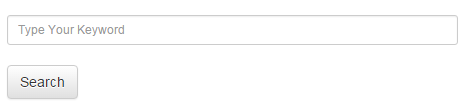
\includegraphics[width=200pt]{search.png}
	\caption{Halaman \textit{search}}
	\label{fig:search}
\end{figure}

\begin{flushleft}
	\textbf{Implementasi Model User}
\end{flushleft}

Pengguna akan menuliskan kata kunci pada search form yang sudah disediakan. Kemudian apabila tombol Search ditekan maka sistem akan melakukan pencarian terhadap kata kunci yang diberikan. Proses pencarian tersebut dilakukan pada data GO dengan menggunakan SPARQL seperti tampak pada Gambar \ref{fig:sparql}.

\begin{figure}[h!] % Gunakan \begin{figure*} untuk memasukkan Gambar
	\centering
	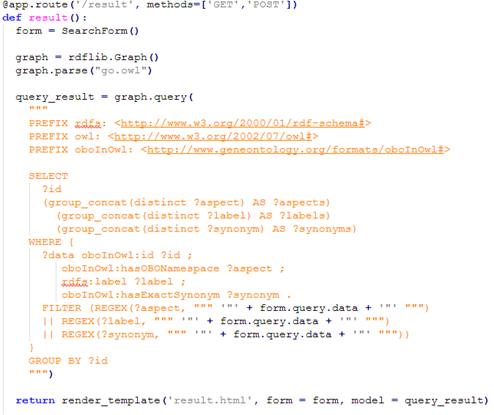
\includegraphics[width=200pt]{sparql.png}
	\caption{\textit{Syntax} proses pencarian \textit{term}}
	\label{fig:sparql}
\end{figure}

Pada Gambar \ref{fig:sparql} terdapat syntax SPARQL, dengan struktur PREFIX dan perintah SELECT. PREFIX digunakan untuk mempersingkat URI yang digunakan pada perintah SELECT. Pada perintah SELECT terdapat bagian yang akan ditampilkan pada halaman web yaitu \textit{?id}, \textit{?aspects}, \textit{?labels} dan \textit{?synonyms}. Kemudian terdapat bagian WHERE menunjukkan variabel apa saja yang akan diambil dari data ontologi. Pada bagian WHERE ini merupakan \textit{triple} yang berupa \textit{subject}, \textit{predicate} dan \textit{object}. \textit{Subject} pada query ini disimbolkan dengan ?data. \textit{Predicate} berupa URI dan atribut yang akan diambil, URI diganti dengan PREFIX agar lebih ringkas dalam penulisannya sebagai contoh oboInOwl:id. \textit{Object} digunakan untuk menyimpan data yang didapat dari hasil query, sebagai contoh \textit{object} ?id. Gambar \ref{fig:result} merupakan hasil dari query yang ditampikan pada halaman result.

\begin{figure}[h!] % Gunakan \begin{figure*} untuk memasukkan Gambar
	\centering
	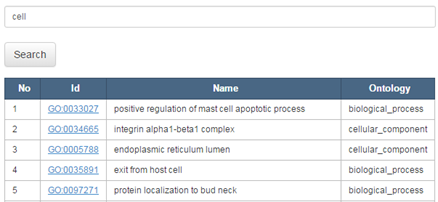
\includegraphics[width=200pt]{result.png}
	\caption{Halaman hasil pencarian \textit{term}}
	\label{fig:result}
\end{figure}
